\documentclass{standalone}
\usepackage{chez}

\begin{document}
\chapter{October 07, 2020}

Last time we saw that the cellular chain complex \(C_*^{\text{cell}}(X)\) of
a CW complex \(X\) computes the singular homology.

\begin{example}[\(S^2\)]
  Let's consider a less-minimal cell structure of \(S^2\) where
  \[
    \Sk_0 S^2 = S^0 \qquad
    \Sk_1 S^2 = S^1 \qquad
    \Sk_2 S^2 = S^2,
  \]
  depicted below.
  \begin{center}
    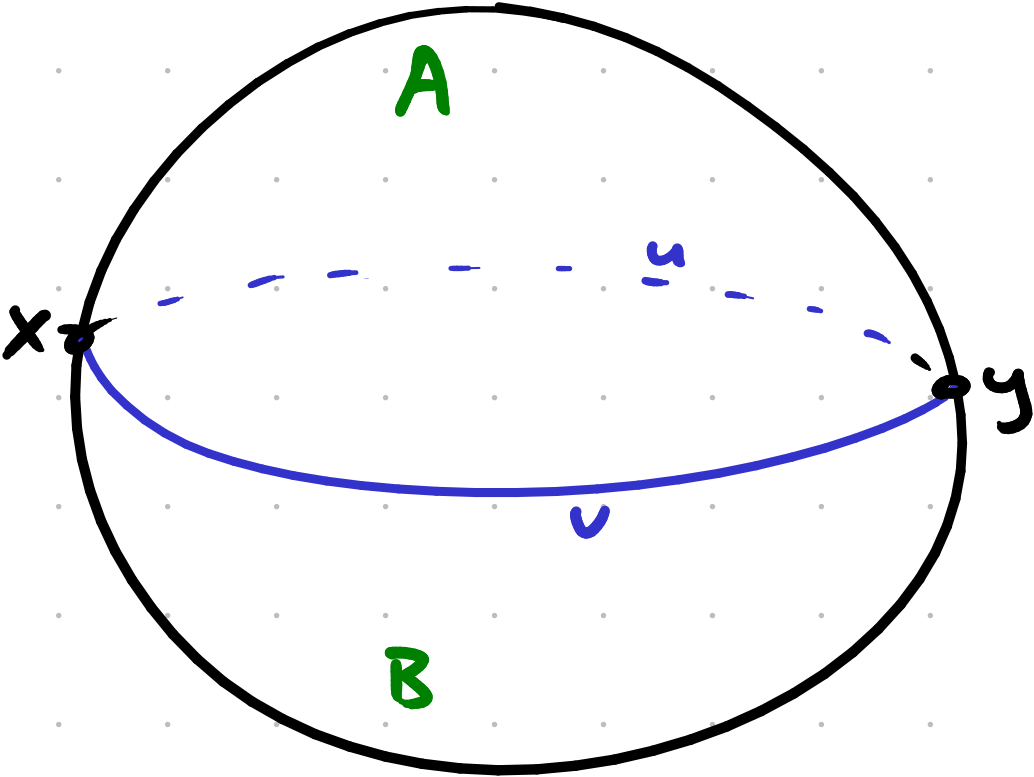
\includegraphics[width=0.2\textwidth]{18_905-201007-1.png}
  \end{center}
  Then
  \[
    C_*^{\text{cell}}(S^2) = \Big({
      \begin{tikzcd}
        \ZZ\fgen{x, y} &
        \ZZ\fgen{u, v} \ar[l, "d"'] &
        \ZZ\fgen{A, B} \ar[l, "d"'] &
        \cdots \ar[l]
      \end{tikzcd}
    }\Big)
  \]
  Note that when we are computing the homology maps,
  we only care about the image of the \(d\) maps.
  In particular, when we are working with semisimplicial sets,
  we cared about the direction that the edges went.
  Here we can make an arbitrary choice of direction to help us
  compute the \(d\) maps.
  In particular, if we select \(x \overset{u}\to y\)
  and \(x \overset{v}\to y\), then
  \[
    du = y - x, \qquad dv = y - x.
  \]
  Then
  \[
    H_0(S^2) = \frac{\ker d}{\img d} = \frac{\ZZ\fgen{x, y}}{\ZZ\fgen{y - x}}
      \iso \ZZ.
  \]

  To determine \(dA\) and \(dB\), note that we can add some maps
  to the pushout diagram of the \(2\)-skeleton
  \[
    \begin{tikzcd}
      S^1 \sqcup S^1 \arrow[r, "f"] \arrow[d, hook] &
        \Sk_1 S^2 \mathrlap{{} = S^1} \arrow[d] \\
      D^2 \sqcup D^2 \arrow[r] &
        \Sk_2 S^2 \mathrlap{{} = S^2}
    \end{tikzcd}
  \]
  Note that the map \(f\) determines \(\Sk_2 S^2\) as the pushout.
  In particular, consider the map
  \[
    \begin{tikzcd}
      S^1 \sqcup S^1 \ar[r] &
      \Sk_1 S^2 \ar[r] &
      \Sk_1 S^2 / \Sk_0 S^2 = S^1 \vee S^1
    \end{tikzcd}
  \]
  Taking \(H_1\), this gives a map
  \[
    \ZZ \oplus \ZZ \to \ZZ \oplus \ZZ
  \]
  that gives the information of \(dA\) and \(dB\),
  since the \(\ZZ\)s on the left represent \(A\) and \(B\),
  and the \(\ZZ\)s on the right represent \(u\) and \(v\).

  In particular, we can again arbitrarily assign
  \[
    dA = u - v, \qquad
    dB = u - v.
  \]
  And indeed, when we compute the homologies from this sequence,
  we get the expected result.

  Moreover, we have that a generator of \(H_2(S^2)\)
  in this CW structure is given by \(A - B\).
  This is because we know \(dA = dB\), since the attaching maps
  \(S^1 \to \Sk_1 S^1\) defining \(A\) and \(B\) are the same.
\end{example}

\subsection{Homotopy equivalence}
Note that homology can be used to prove that topological spaces
are not homotopy equivalent.
In particular, this is just a consequence of homology
being an invariant under homology.

A less obvious statement is that homology can also be used
to prove that continuous maps are not homotopic.
Homology is a functor, so it takes maps in \(\cTop\) to maps in \(\cAb\).
So, if two continuous maps are sent to different maps of abelian groups,
then the two continuous maps cannot be homotopic.

\begin{definition}
  If \(f \colon S^n \to S^n\) is a continuous map,
  then the \vocab{degree} of \(f\), denoted \(\deg f\), is the value of \(1\)
  under the group homomorphism \(H_n(f) \colon \ZZ \to \ZZ\).
\end{definition}

If \(f, g \colon S^n \to S^n\) are two continuous maps that
have different degrees, then \(f\) and \(g\) are hot homotopic,
as otherwise \(H_n(f) = H_n(g)\).

\begin{lemma}
  Suppose \(f, g \colon S^n \to S^n\). Then
  \[
    \deg (g \circ f) = (\deg g)(\deg f).
  \]
\end{lemma}
\begin{proof}
  Consider the diagram
  \[
    \begin{tikzcd}
      S^n \ar[r, "f"] &
      S^n \ar[r, "g"] &
      S^n
    \end{tikzcd}
  \]
  When we apply \(H_n\), we get
  \[
    \begin{tikzcd}[row sep=0.15]
      \ZZ \ar[r, "H_n(f)"] &
        \ZZ \ar[r, "H_n(g)"] &
        \ZZ \\
      1 \ar[r, mapsto] & \deg f \\
      & 1 \ar[r, mapsto] & \deg g \\
      1 \ar[rr, mapsto] & & (\deg f)(\deg g)
    \end{tikzcd}
  \]
\end{proof}

\begin{corollary}
  Suppose \(f \colon S^n \to S^n\) is a homeomorphism.
  Then \(\deg f\) is either \(1\) or \(-1\).
\end{corollary}

\begin{example}
  Consider the map \(f \colon S^2 \to S^2\) that is
  a reflection about a plane.
  Note that \(f\) is also a map of CW complexes.
  If we select the skeleta such that the plane of reflection is the equator,
  then we know that \(A\) and \(B\) have the same boundary, and the map
  \[
    S^1 \sqcup S^1 \to \Sk_1 S^2 \to \Sk_1 S^2 / \Sk_0 S^2 \iso S^1 \vee S^1
  \]
  sends the boundaries of \(A\) and \(B\) to the same set.
  In particular, we know that \(d A = d B\), so
  \[
    A - B \in \ker d = H_2^{\text{cell}}(S^2) \iso \ZZ.
  \]
  Therefore, \(A - B\) is a generator of \(H_2^{\text{cell}}(S^2)\).
  In particular, \(f\) is the map between the cellular complexes
  \[
    \begin{tikzcd}
      \ZZ\fgen{A, B} \arrow[r]
        \arrow[d, "A \mapsto B" pos=0.2, "B \mapsto A" pos=0.6] &
        \ZZ\fgen{u, v} \arrow[r]
          \arrow[d, "u \mapsto u" pos=0.2, "v \mapsto v" pos=0.6] &
        \ZZ\fgen{x, y}
          \arrow[d, "x \mapsto x" pos=0.2, "y \mapsto y" pos=0.6] \\
      \ZZ\fgen{A, B} \arrow[r] &
        \ZZ\fgen{u, v} \arrow[r] &
        \ZZ\fgen{x, y}
    \end{tikzcd}
  \]
  This means \(f \colon A - B \mapsto B - A\),
  so \(H_2(f) \colon \ZZ \to \ZZ\) is multiplication by \(-1\).
  Therefore, \(f\) has degree \(-1\).
\end{example}
Note that this argument also works for \(S^n\) in general,
so no reflection \(S^n \to S^n\) is homotopic to the identity.

\begin{corollary}
  The degree of a rotation of \(S^n\) is \(1\).
\end{corollary}
This is because any rotation can be written as
the composition of two reflections.

\begin{example}
  \begin{itemize}[nosep]
    \item The degree of \(S.to S^1\) where \(x \mapsto -x\) is \(1\) because
          it is a \(180^\circ\) rotation.
    \item We can find he degree of \(S^2 \to S^2\) where \(x \mapsto -x\)
          by considering the map as the composite of three reflections
          \[
            (a, b, c) \mapsto (-a, b, c)
                      \mapsto (-a, -b, c)
                      \mapsto (-a, -b, -c).
          \]
          Therefore, this map has degree \(-1\).
    \item More generally, the antipodal map \(S^n \to S^n\)
          mapping \(x \mapsto -x\) is the composite of \(n+1\) reflections,
          so the map has degree \((-1)^{n+1}\).
  \end{itemize}
\end{example}





\end{document}
